\documentclass[../notes.tex]{subfiles}
\graphicspath{{\subfix{../img/}}}
\begin{document}

\section{Goals of Control Theory}
Control theory is a branch of engineering that deals with the behavior of dynamical systems and how to influence that behavior through inputs. Typical considerations are:
\begin{description}
    \item[Stability] Ensuring the system remains bounded and predictable over time, and preventing oscillations or otherwise chaotic behavior.
    \item[Controllability] Determining whether a system can be driven from an initial state to a desired final state using the available control inputs.
    \item[Observability] Assessing how much of the internal state of a system can be inferred from its outputs. Crucial for systems where direct measurement of all variables isn't possible.
    \item[Optimality] Achieving the desired behavior with minimal cost (energy, time). Involves balancing between speed, accuracy, and resource usage.
    \item[Robustness] Maintaining performance despite uncertainties, disturbances, or modelling inaccuracies. The controller must be able to handle real world imperfections!
    % \item[Feedback Design] Correcting errors and adapting to changes
\end{description}

\begin{figure}[H]
    \centering
    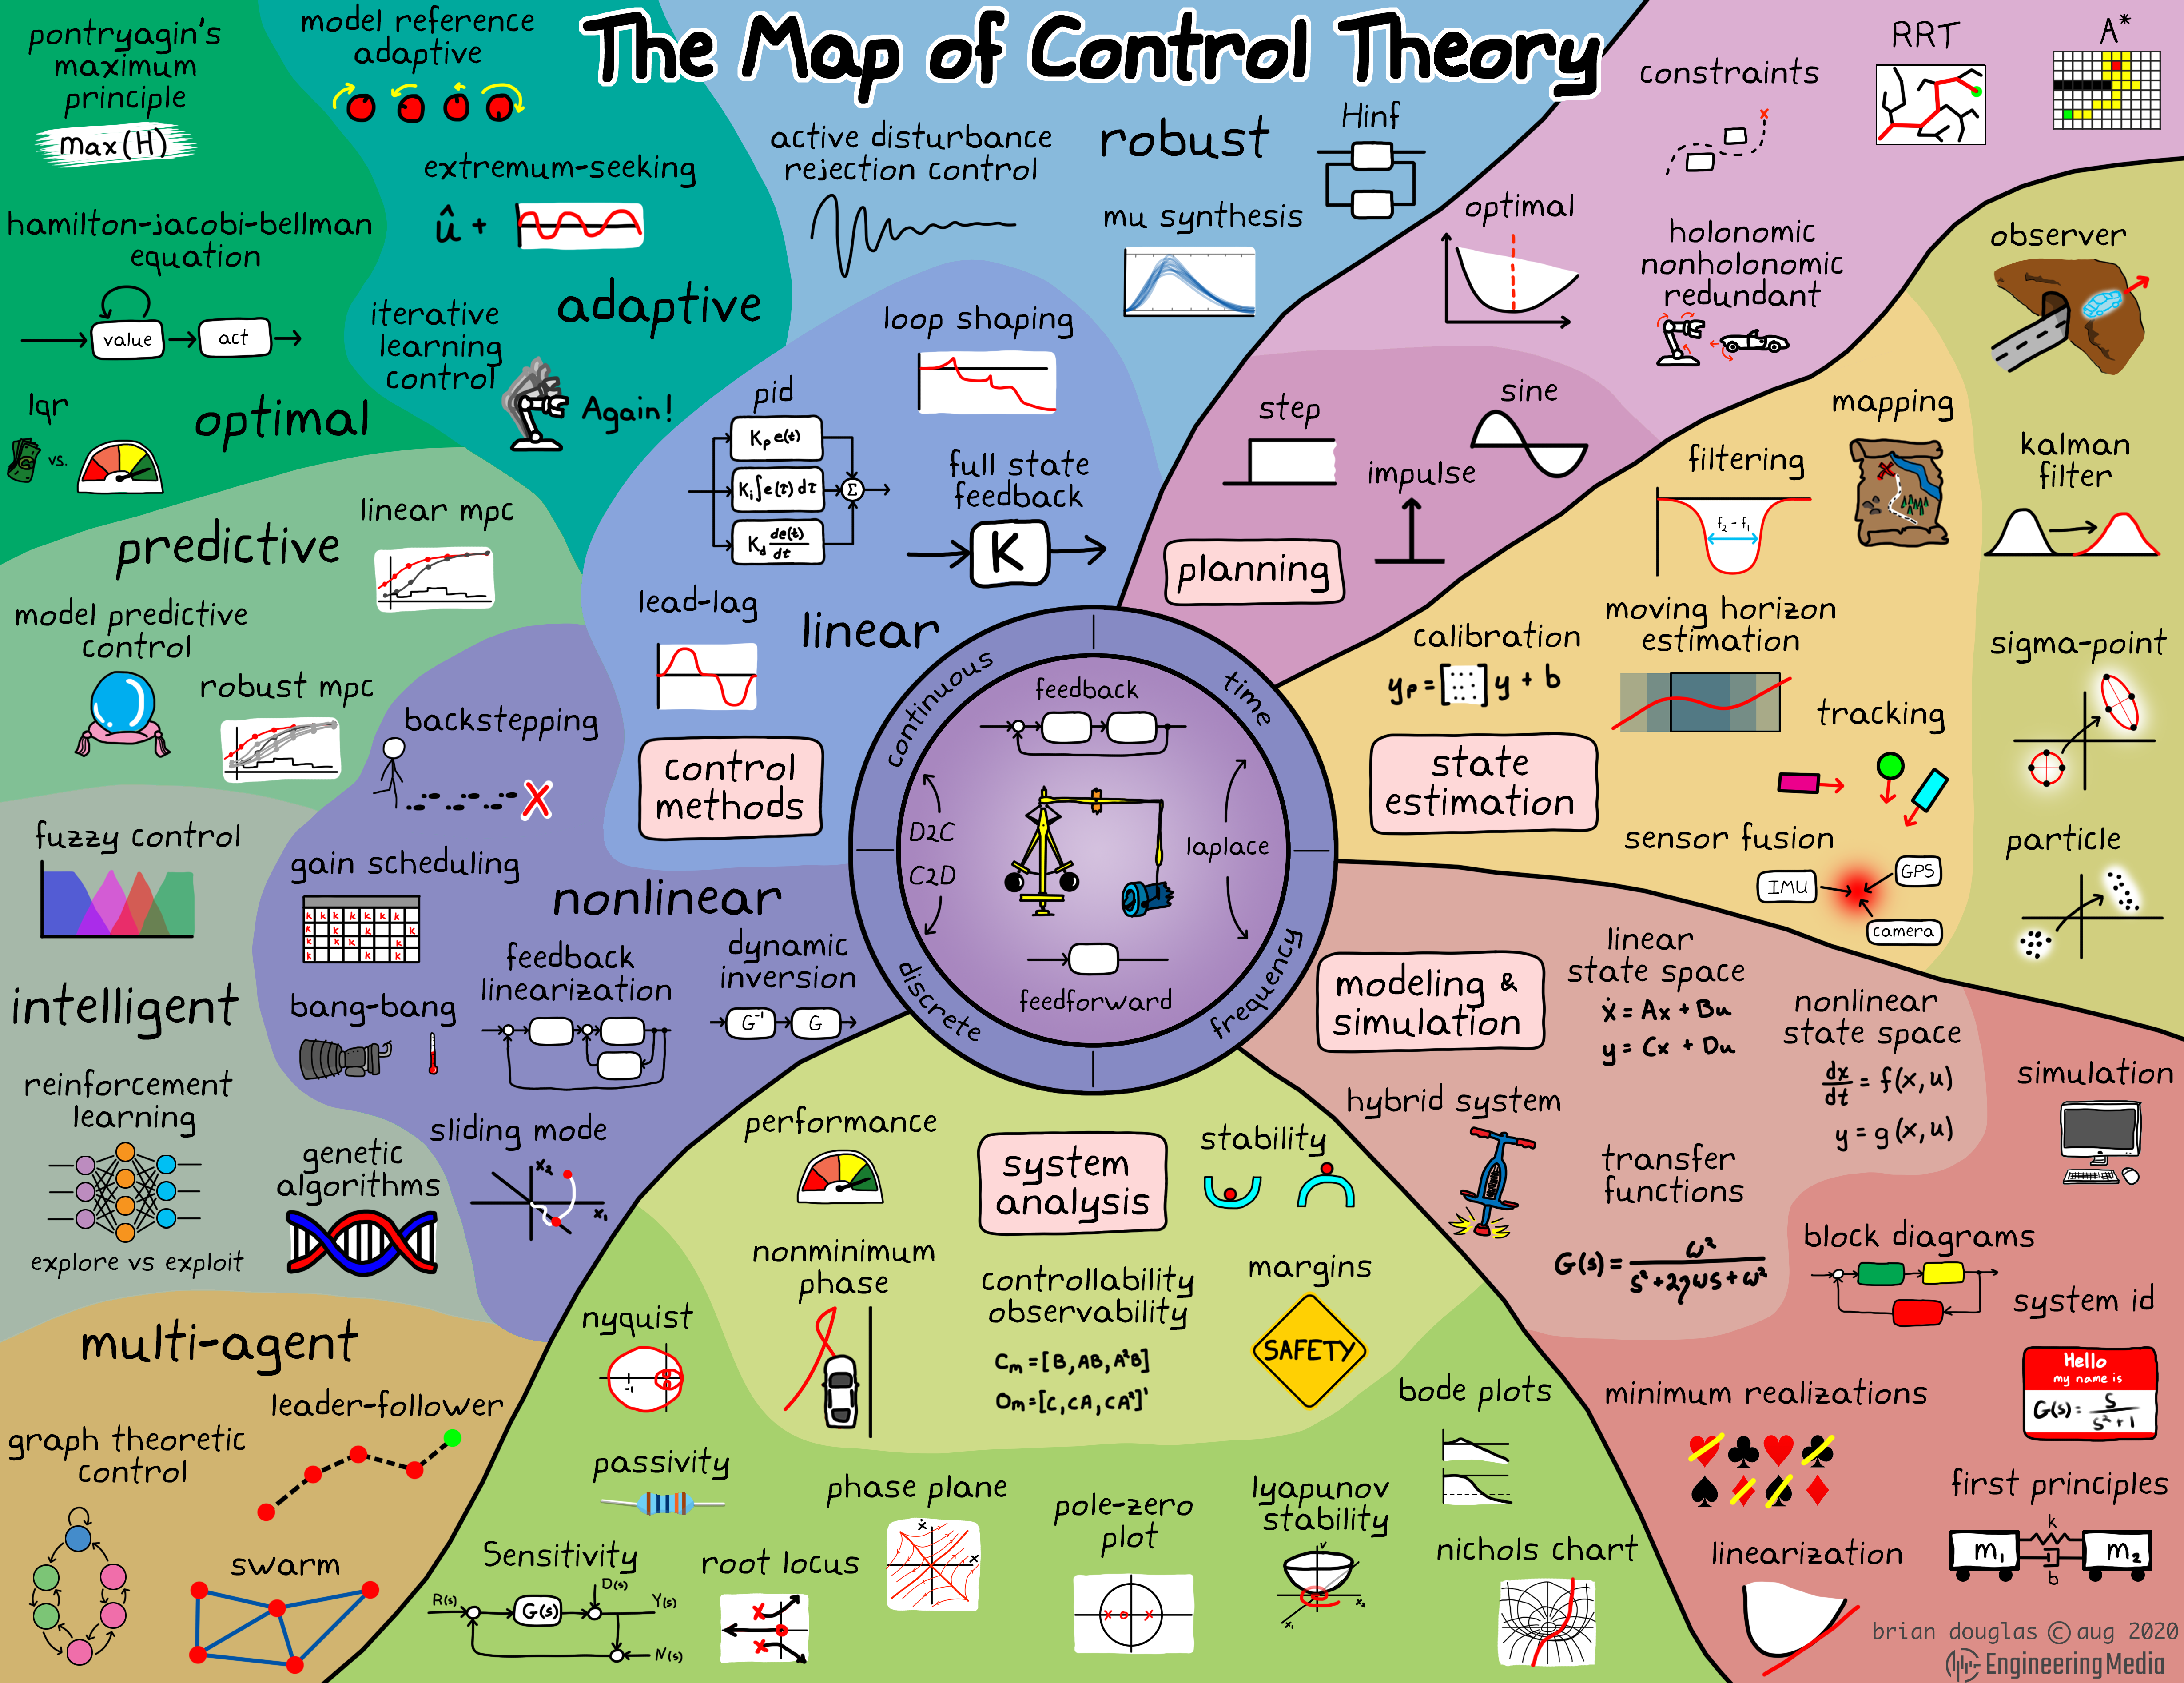
\includegraphics[width=1\linewidth]{Control_Map.png}
    \caption{Brian Douglas' Concept Map of Control Theory}
    \label{fig:controlMap}
\end{figure}

Control theory is a interdisciplinary topic. It can be applied to mechanical, electrical, thermal, fluid, really any system. Examples include a swinging pendulum, predator v.s. prey dynamics, RLC circuits, mass-spring-damper systems, etc.

\subsection{Applications to Aerospace}
The main application of control theory in aerospace is in Guidance, Navigation, and Control (GNC). In order from most broad to least:
\begin{description}
    \item[Navigation (Statistics)] "Given the measurements we have, where do we think we are?"
    \item[Guidance (Optimization)] "Given where we want to go and where we think we are, which path should we follow?"
    \item[Control (Differential Equations)] "What effort should we apply and how should we control actuators given where we are and the chosen path?"
\end{description}
All require knowledge of dynamics and linear algebra, and can be further broken down into numerous subcategories.\\ 
Control theory offers many benefits in the aerospace application. 
\begin{description}
    \item[Automation] Remove the need for human intervention, preserving the attention of the operator for more important matters.
    \item[Performance] Operate more effectively than a human operator.
    \item[Safeguards / Protections] Prevent the craft from exceeding design limits.
    \item[Deferred Decision-making] Let the human operator make certain flight critical decisions.
\end{description}

\subsection{Timeline of Development}
\paragraph{Classical Control (prior to 1950's)}
\begin{itemize}
    \item Analysis of linear control systems.
    \item Controller design using frequency domain representation.
\end{itemize}
\paragraph{Advanced Topics (post 1950's)}
\begin{itemize}
    \item Multivariable systems (state domain representation).
    \item Nonlinear and adaptive control.
    \item Optimal control.
    \item Estimation and filtering.
    \item Stochastic control and reinforcement learning.
\end{itemize}

\subsection{Examples of Control Systems}
\paragraph{Falcon 9 Landing}
An example of controlling an inverted pendulum. Following a flight trajectory (actual vs desired path).
\paragraph{X-29 jet}
Unstable design leads to control difficulties, but also results in high manueverability.

\subsection{Common Definitions}
\begin{description}
    \item[Dynamical System] A collection of quantities / variables with significance that change over time due to interactions with each other and the environment. Typical form: $\dot{x} = f(x)$. 
    \item[Dimension] The number of quantities / variables to model. There are infinite dimensional systems as well, for example fluid flow. 
\end{description}

\end{document}